\chapter{ Aufbau der optischen Diode}

Um eine destabilisierende Rückkopplung in den He-Ne-Resonator zu verhindern, setzen wir den Isolator ein, der im \cref{fig:function_of_optical_diode} dargestellt ist. 
Brewster-Fenster, so angebracht, dass sie im Brewster-Winkel \cite{introtoED} 
\begin{equation}
  \tan\theta_B = \bigl(\tfrac{n_{\mathrm{glas}}}{n_{\mathrm{luft}}}\bigr),
\end{equation}
stehen, dienen als erster Polarisationsfilter innerhalb der Kavität. 
Bei diesem Winkel passiert p-polarisiertes Licht (mit elektrischem Feld in der Einfallsebene) die Glas-Luft-Grenzfläche ohne Reflexion, während s-polarisiertes Licht (Feld senkrecht zur Einfallsebene) teilweise reflektiert und somit unterdrückt wird. 
Dadurch ist der intra-kavitär austretende Strahl am Ausgangskoppler bereits stark linear entlang der p-Achse polarisiert und liefert einen sauberen Eingangsstatus für die nachfolgenden Isolator-Komponenten.

\begin{figure}[htbp]
  \centering
  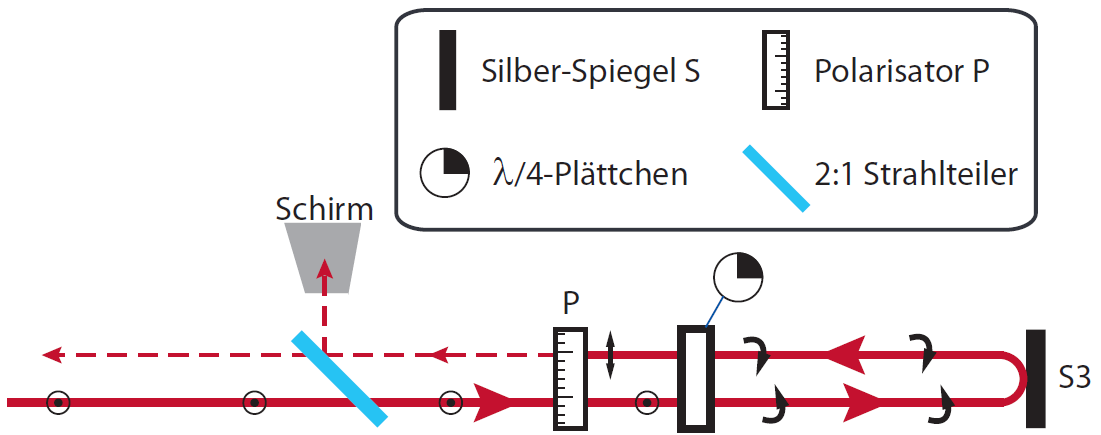
\includegraphics[width=0.75\linewidth]{Funktion der optischen Diode.png}
  \caption{Funktionsprinzip des optischen Isolators: Der rückwärts laufende Strahl ist zur Veranschaulichung leicht versetzt dargestellt. Schwarze Pfeile entlang des Strahlengangs zeigen mögliche Polarisationszustände in den einzelnen Stufen an. \cite{praktikum}}
  \label{fig:function_of_optical_diode}
\end{figure}

Der Isolator selbst besteht aus einem linearen Polarisator (P), einer Viertelwellenplatte ($\lambda/4$) und einem Silber-Spiegel (S3), die unmittelbar hinter dem Ausgangskoppler in Serie angeordnet sind (siehe \cref{fig:aufbau_mit_optischer_diode}). 
Auf dem Vorwärtsdurchgang überträgt P nur das p-polarisierte Licht, welches die $\lambda/4$-Platte in rechtszirkulare Polarisation umwandelt. 
Nach der Reflexion an S3 - die Drehrichtung beibehält - durchläuft der Rückstrahl erneut die $\lambda/4$-Platte und tritt als um 90° gedrehtes, nun s-polarisiertes Licht aus. 
Dieses gedrehte Licht wird von P blockiert, sodass eine hohe nicht-reziproke Isolation erreicht wird, ohne nennenswerte Einfügedämpfung im Vorwärtsweg.
\begin{figure}[htbp]
  \centering
  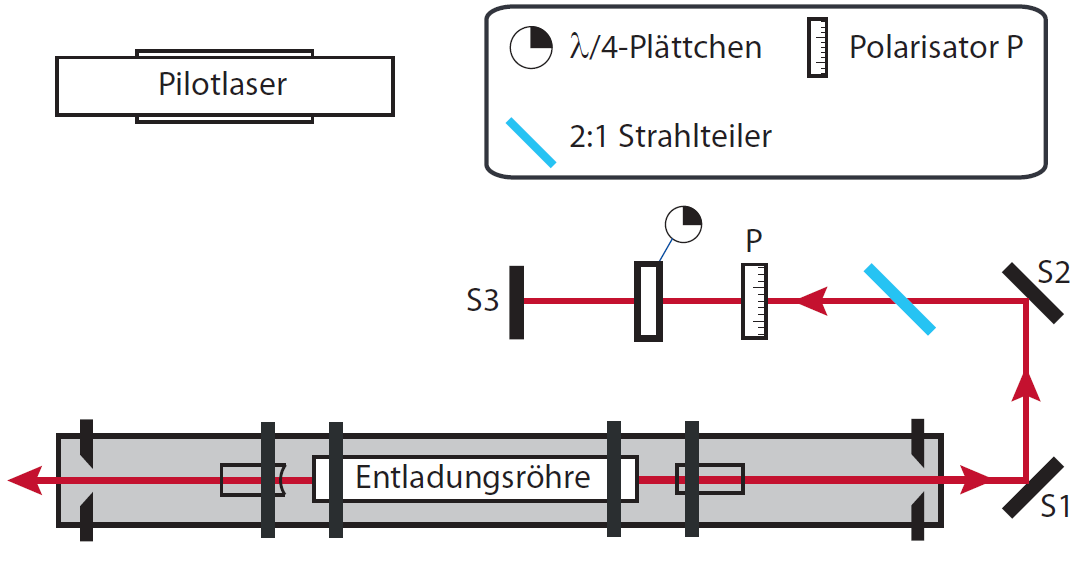
\includegraphics[width=0.75\linewidth]{Aufbau mit optischer Diode.png}
  \caption{Aufbau mit optischer Diode \cite{praktikum}}
  \label{fig:aufbau_mit_optischer_diode}
\end{figure}

Mechanisch sind der Polarisator, die $\lambda/4$-Platte und ein nicht-polarisierender Strahlteiler im Verhältnis 2 : 1 in Justierhaltern montiert, die feines Kippen und Drehen sowie axiale Ausrichtung erlauben. 
Der Strahlteiler führt etwa ein Drittel des Vorwärtslichts zu einer Leistungsüberwachung ab, während der Rest zur schnellen Photodiodenkette gelangt. Alle Optiken verfügen über breitbandige Antireflexbeschichtungen, um Streureflexionen zu minimieren.

\paragraph{Justage-Prozedur:}
\begin{enumerate}
  \item \textbf{Polarisator-Orientierung:} Um die native p-Polarisation des Lasers einzustellen, wird P gedreht, bis die durch den Monitorport gemessene Leistung maximal ist.
  \item \textbf{Viertelwellenplatten-Einstellung:} S3 wird entfehrnt und  die $\lambda/4$-Platte justiert, bis die schwache Rückreflexion durch P auf einem Schirm verschwindet - dies ist ein Zeichen für eine perfekte 90°-Drehung der rücklaufenden Polarisation.
  \item \textbf{Isolations-Überprüfung:} S3 wird wieder eingesetzt und es wird geprüft, dass kein messbarer Rückfluss durch P auftritt, während die Vorwärtsdurchlässigkeit unverändert bleibt.  
\end{enumerate}
Während der Justage wurde der Polarisator auf $\theta = 290^\circ \pm 1^\circ$ und die Viertelwellenplatte auf $\lambda/4 = 64^\circ \pm 1^\circ$ eingestellt.


%===============================================================================================================================================================================================================================================================================================================================================
\chapter{Optischer Spektrumanalysator} \label{sec:5.7}

Nach Verlassen des Isolators wird der He-Ne-Strahl in einen konfokalen Fabry-Perot-Resonator (\cref{fig:Spektrumanalysator}) mit äußerer Länge $l_{\mathrm{ext}} = 5{,}0\,\si{\centi\meter}$ eingekoppelt. \\
Nach Handbuch \cite{praktikum} sind dessen Eigenfrequenzen
\begin{equation}
  \nu_{qnm}
  = \Bigl(q + \tfrac{m+n+1}{2}\Bigr)\,\frac{c}{2\,l} .
\end{equation}
Gleiche transversale Moden TEM$_{nm}$ liegen damit im Abstand des freien Spektralbereichs
\begin{equation*}
  \Delta\nu_{\mathrm{FSR}}
  = \frac{c}{2\,l},
\end{equation*}
während benachbarte Moden um
\begin{equation*}
  \Delta\nu
  = \frac{c}{4\,l}
\end{equation*}
getrennt sind.
\begin{figure}[htbp]
  \centering
  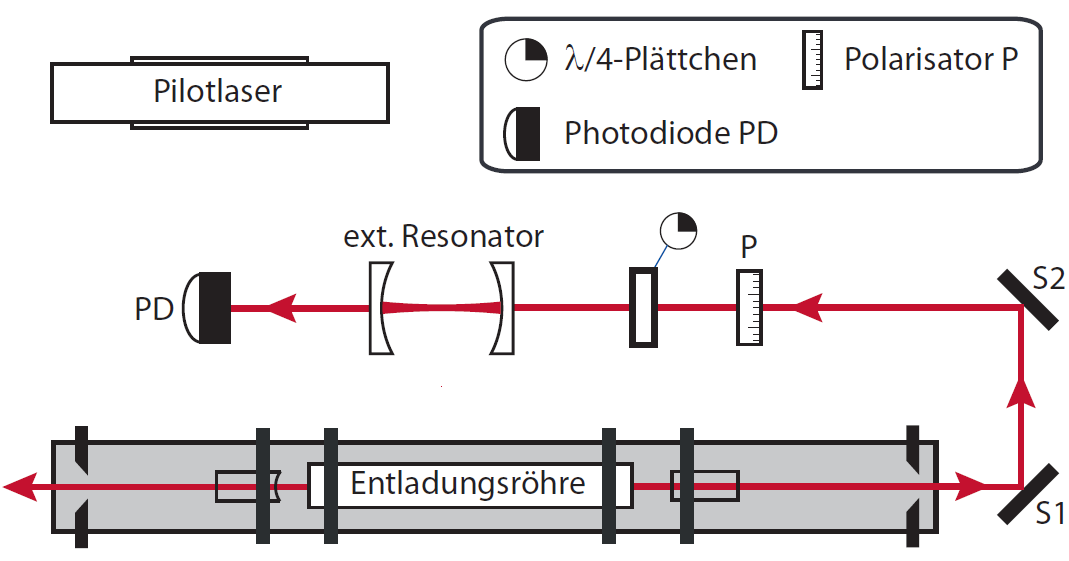
\includegraphics[width=0.75\linewidth]{Aufbaus zum optischen Spektrumanalysator.png}
  \caption{Schema des Aufbaus zum optischen Spektrumanalysator \cite{praktikum}}
  \label{fig:Spektrumanalysator}
\end{figure}

Ein Piezoaktor verändert $l_{\mathrm{ext}} = 5 \si{\cm}$ um etwa $200\,\si{\nm}$ bei einer $0-100 \si{\volt}  $/$50 \si{\hertz}$-Dreiecksspannung, so dass ein vollständiger Sweep genau eine $\Delta\nu_{\mathrm{FSR}}$ abtastet. 
Kanal 1 des Oszilloskops zeigt die Piezo-Spannung $U(t)$, Kanal 2 die transmittierte Intensität $I(t)$ einer langsamen Photodiode, was eine Folge von Übertragungsclustern wie zwischen \cref{fig:9a} bis \cref{fig:9c} ergibt. 
Die korrekte Justage erfolgte mittels Papierziel- und Zwei-Spiegel-Kippverfahren (\cref{fig:Resonator}), bis für jede Piezo-Position ein einziger scharfer Spot auftrat und die Peaks minimal verbreitert waren.
\begin{figure}[htbp]
  \centering
  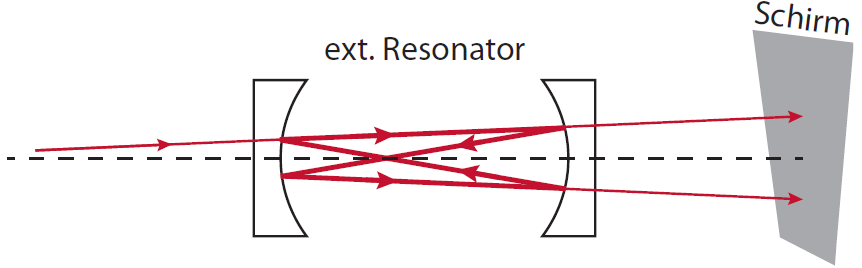
\includegraphics[width=0.75\linewidth]{Resonator bei Dejustage.png}
  \caption{Strahlengang im externen Resonator bei Dejustage \cite{praktikum}}
  \label{fig:Resonator}
\end{figure}
\begin{figure}[htbp]
    \centering
    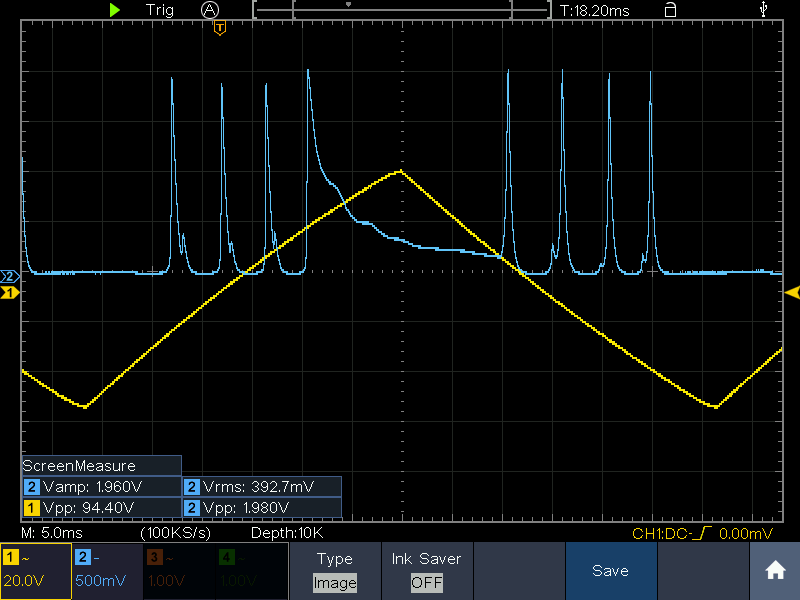
\includegraphics[width=0.75\linewidth]{52_1a.png}
     \caption{Oszilloskopübertragungscluster interne Kavitätenlängen $l = 52,0\,\si{\centi\meter} \pm$ 0{,}4\,\si{\centi\meter}.}
    \label{fig:9a}
\end{figure}
  \begin{figure}[htbp]
    \centering
    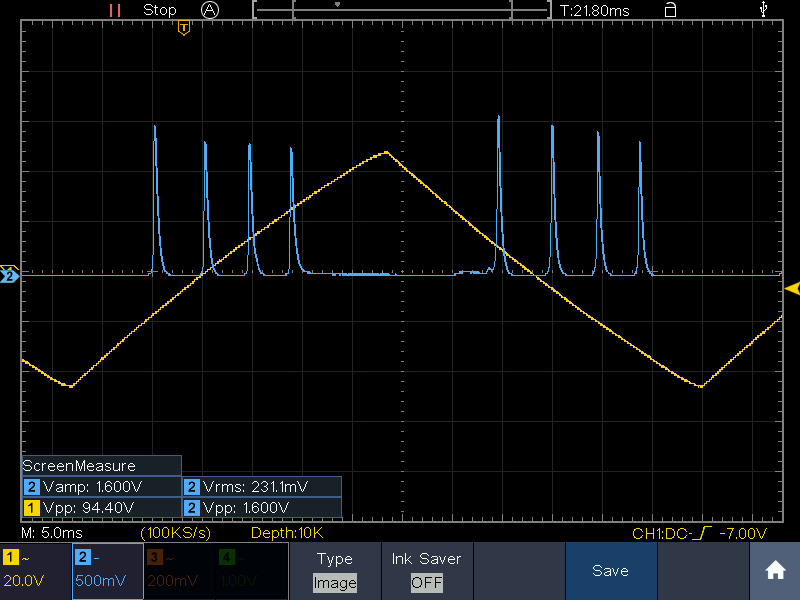
\includegraphics[width=0.75\linewidth]{68_1a.png}
     \caption{Oszilloskopübertragungscluste interne Kavitätenlängen $l = 68,0\,\si{\centi\meter} \pm$ 0{,}3\,\si{\centi\meter}.}
    \label{fig:9b}
  \end{figure}
  \newpage
  \begin{figure}[htbp]
    \centering
    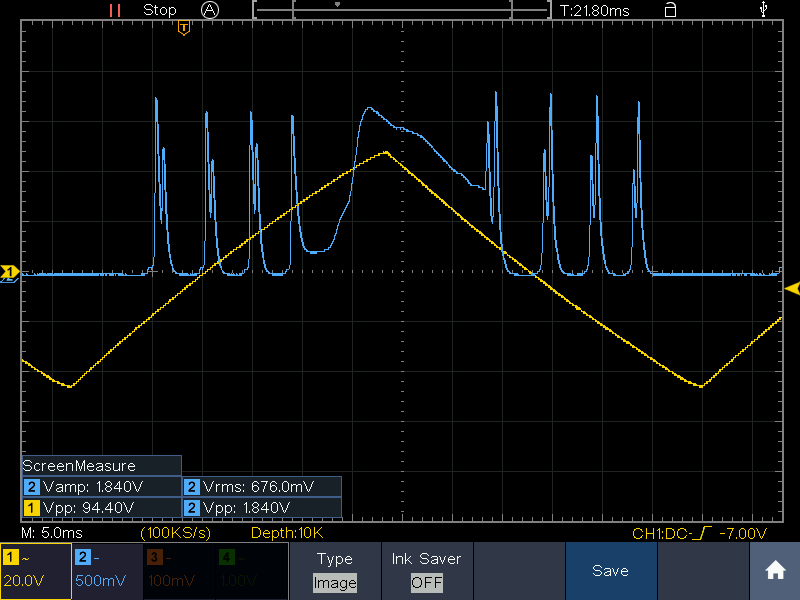
\includegraphics[width=0.75\linewidth]{80_1a.png}
     \caption{Oszilloskopübertragungscluster interne Kavitätenlängen $l = 80,0\,\si{\centi\meter} \pm$ 0{,}3\,\si{\centi\meter}.}
    \label{fig:9c}
  \end{figure}
 
 Für jede Oszilloskop-Spur bestimmen wir zwei Zeitintervalle: $a$, die horizontale Ausdehnung eines gesamten Übertragungsclusters (entspricht einer freien Spektralbreite des externen Fabry-Perot-Analysators), und $b$, der Abstand zweier benachbarter Peaks innerhalb dieses Clusters (entspricht dem longitudinalen Modenabstand der internen He-Ne-Kavität). 
 Da sowohl $a$ als auch $b$ auf derselben (möglicherweise nichtlinearen) Piezo-Zeitachse abgelesen werden, kompensiert ihr Verhältnis jede unbekannte Kalibrierkonstante. Damit lassen sich drei Frequenzintervalle definieren.

Die freie Spektralbreite des Analysators ist
\begin{equation}
  \Delta\nu_{\mathrm{FSR}}
  = \frac{c}{2\,l_{\mathrm{ext}}}
  = \frac{299\,792\,458\;\mathrm{m/s}}{2 \times 0{,}050\;\mathrm{m}}
  \approx 3{,}00\;\mathrm{GHz},
\end{equation}
wobei $l_{\mathrm{ext}} = 5{,}0\;\mathrm{cm}$.

Der experimentell bestimmte Modenabstand des Lasers ergibt sich zu
\begin{equation}
 \Delta\nu_{\mathrm{exp}}
  = \frac{b}{a}\;\Delta\nu_{\mathrm{FSR}},
\end{equation}
mit der Fehlerfortpflanzung
\begin{equation}
  \delta\Delta\nu_{\mathrm{exp}}
  =\Delta\nu_{\mathrm{exp}}
    \sqrt{\Bigl(\frac{\delta b}{b}\Bigr)^{2}
        + \Bigl(\frac{\delta a}{a}\Bigr)^{2}
        + \Bigl(\frac{\delta l}{l}\Bigr)^{2}}\!,
\end{equation}
wobei die Cursor-Unsicherheiten $\delta a = 0{,}20\;\mathrm{ms}$ und $\delta b = 0{,}20\;\mathrm{ms}$ sowie die Längenunsicherheiten $\delta l_{52} = 0{,}4\;\mathrm{cm}$ und $\delta l_{68} = \delta l_{80} = 0{,}3\;\mathrm{cm}$ betragen.

Der theoretische Modenabstand für eine ideale planparallele Kavität der Länge $l$ ist
\begin{equation}
 \Delta\nu_{\mathrm{theo}}
  = \frac{c}{2\,l},
  \quad
  \delta\Delta\nu_{\mathrm{theo}}
  =\Delta\nu_{\mathrm{theo}}\,\frac{\delta l}{l}.
\end{equation}

\begin{table}[H]
  \centering
  \resizebox{0.8\columnwidth}{!}{%
    \begin{tabular}{|c|c|c|c|c|}
      \hline
      $l \,\;\pm\delta l \,/\mathrm{cm}$ 
        & $a \,\pm \delta a\,/\mathrm{ms}$ 
        & $b \,\pm \delta b\,/\mathrm{ms}$ 
        & $v_{\mathrm{exp}}\pm\delta\Delta\nu_{\mathrm{exp}}\;/\;\mathrm{MHz}$ 
        & $v_{\mathrm{theo}}\pm\delta\Delta\nu_{\mathrm{theo}}\;/\;\mathrm{MHz}$ \\ \hline
      $52{,}0 \pm 0{,}4$   & $25{,}0 \pm 0{,}2$ & $3{,}0 \pm 0{,}2$ & $360 \pm 13$ & $288 \pm 2$ \\ \hline
      $68{,}0 \pm 0{,}3$   & $25{,}0 \pm 0{,}2$ & $2{,}0 \pm 0{,}2$ & $240 \pm 12$ & $220 \pm 1$ \\ \hline
      $80{,}0 \pm 0{,}3$   & $25{,}0\pm 0{,}2$ & $1{,}5 \pm 0{,}2$ & $180 \pm 12$ & $187 \pm 1$ \\ \hline
    \end{tabular}%
  }
  \caption{Experimentelle und theoretische Modenabstände für drei interne Kavitätenlängen.}
  \label{tab:mode-spacings}
\end{table}

Der Modenabstand nimmt proportional zu $1/l$ ab, wie genau vorhergesagt. 
Für $l = 68\,\mathrm{cm}$ und $l = 80\,\mathrm{cm}$ liegen die experimentellen Werte innerhalb ihrer kombinierten Unsicherheiten mit den theoretischen Vorhersagen überein, was sowohl die Kalibrierung des Analysators als auch die Gültigkeit der einfachen Formel$ \frac{c}{2\,l}$ für den Laser bestätigt. 
Die Messung bei $l = 52\,\mathrm{cm}$ weicht um etwa 25\,\% ab, höchstwahrscheinlich, weil der Cursor für $b$ zwischen nicht-benachbarten Peaks gesetzt oder die Clustergrenze für $a$ falsch identifiziert wurde; eine Wiederholung dieser Aufnahme mit verfeinerter Cursor-Positionierung sollte sie in Übereinstimmung mit den anderen beiden Ergebnissen bringen.

Die Unsicherheiten werden hauptsächlich durch die Cursor-Platzierung und die mit dem Maßband bestimmte Längenunsicherheit $\delta l$ dominiert. Systematische Fehler wie Piezo-Hysterese oder Nichtlinearität der Sweep-Geschwindigkeit heben sich im Verhältnis $b/a$ auf, während verbleibende Spiegel-Dejustagen durch iteratives Feinkippen unterdrückt wurden, bis keine weitere Verengung der Peak-Breiten möglich war. Zukünftige Verbesserungen sind straightforward: Das Speichern der Rohspuren als CSV-Dateien ermöglicht Lorentz-Fits, die $\delta a$ und $\delta b$ auf unter $0{,}02\,\mathrm{ms}$ reduzieren würden, und der Ersatz des Maßbands durch einen Messschieber ($\pm .05 \si{/cm}$) würde $\delta l / l$ in den $10^{-3}$-Bereich senken. Mit diesen Optimierungen sollten alle drei Kavitätenlängen das Gesetz $1/l$ auf besser als 1\,\% bestätigen und eine noch genauere Überprüfung der Analysator-Kalibrierung liefern.



%===============================================================================================================================================================================================================================================================================================================================================
\chapter{ Präzise Messung des Modenabstandes mittels einer
optischen Schwebung} \label{sec:5.8}

Nach der optischen Bestimmung des Modenabstands in \cref{sec:5.7} wird dieselbe Größe nun auf einer absoluten RF-Skala gemessen, indem zwei longitudinale Moden auf einer schnellen Photodiode überlagert und das Misch-IF-Signal auf einem 350 MHz-Oszilloskop analysiert wird \cref{fig:difffreq}. Zwei benachbarte Kavitätsfrequenzen $\nu_{1} = \omega_{1}/2\pi$ und $\nu_{2} = \omega_{2}/2\pi$ erzeugen nach quadratischer Detektion einen RF-Term bei der Differenzfrequenz
\begin{equation*}
  \Delta\omega = \omega_{1} - \omega_{2} = 2\pi\,\Delta\nu_{\mathrm{beat}},
\end{equation*}
wobei alle hochfrequenten Summen- und $2\omega$-Terme oberhalb der 35 MHz-Low-Pass-Grenze des Mixers liegen und somit unterdrückt werden. Die ganze Zahl $m$ bezeichnet die Anzahl der longitudinalen Intervalle zwischen den beiden Moden ($m=1$ für benachbarte Moden, $m=2$ für jeden zweiten Modenabstand usw.), sodass gilt
\begin{equation}
  \Delta\nu_{\mathrm{beat}} = m\,\Delta\nu_{\mathrm{laser}}.
\end{equation}

\begin{figure}[htbp]
    \centering
    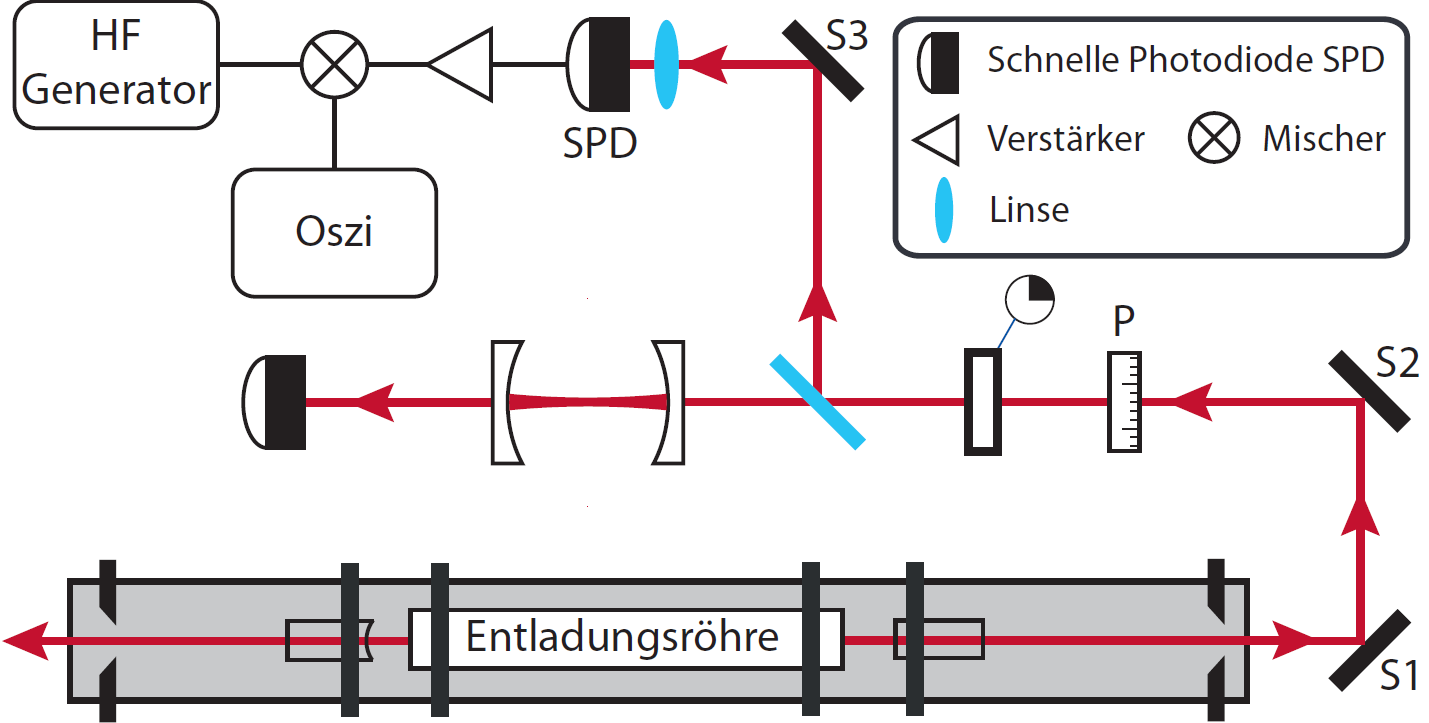
\includegraphics[width=0.75\linewidth]{Differenzfrequenz verschiedener.png}
     \caption{Schematischer Aufbau zur präzisen Messung der Differenzfrequenz verschiedener longitudinaler Moden \cite{praktikum}}
    \label{fig:difffreq}
  \end{figure}

Der IF-Ton $f$ wurde mit Oszilloskop-Cursorn abgelesen; seine Halbwertsbreite (HWHM) liefert die statistische Unsicherheit $\delta f$. Für unsere Spuren beträgt HWHM etwa $0{,}10\,\mathrm{MHz}$ für $m=1$ und $0{,}50\,\mathrm{MHz}$ für $m=2$. Der experimentelle Modenabstand ergibt sich zu
\begin{equation}
  \Delta\nu_{\mathrm{exp}} = \frac{f}{m}, 
  \qquad
  \delta(\Delta\nu_{\mathrm{exp}}) = \frac{\delta f}{m}.
\end{equation}

Der theoretische Modenabstand einer idealen planparallelen Kavität der Länge $l$ lautet
\begin{equation}
  \Delta\nu_{\mathrm{theo}} = \frac{c}{2\,l}, 
  \qquad
  \delta(\Delta\nu_{\mathrm{theo}}) = \Delta\nu_{\mathrm{theo}}\,\frac{\delta l}{l},
\end{equation}
mit $c = 299\,792\,458\;\mathrm{m/s}$. Die Längen wurden mit einem Stahlmaßband gemessen; $\delta l_{52} = 0{,}4\,\mathrm{cm}$ und $\delta l_{68,70.8,80} = 0{,}3\,\mathrm{cm}$.

\begin{table}[H]
  \centering
  \resizebox{0.8\columnwidth}{!}{%
    \begin{tabular}{|c|c|c|c|c|}
      \hline
      $l \pm \delta l \;/\si{\centi\meter}$ & $m$ & $f\; \pm \delta f\;/\si{\mega\hertz}$ &
      $\Delta\nu_{\mathrm{exp}}\pm\delta(\Delta\nu_{\mathrm{exp}})\;/\si{\mega\hertz}$ &
      $\Delta\nu_{\mathrm{theo}}\pm\delta(\Delta\nu_{\mathrm{theo}})\;/\si{\mega\hertz}$ \\ \hline
      $52{,}0\pm0{,}4$ & 1 & $303{,}7  \pm 0{,}10$ & $303{,}7\pm0{,}10$ & $288{,}3\pm2{,}2$ \\ \hline
      $68{,}0\pm0{,}3$ & 1 & $135{,}7  \pm  0{,}10 $ & $135{,}7\pm0{,}10$ & $220{,}4\pm1{,}0$ \\ \hline
      $68{,}0\pm0{,}3$ & 2 & $309{,}9  \pm  0{,}50 $ & $154{,}9\pm0{,}25$ & $220{,}4\pm1{,}0$ \\ \hline
      $70{,}8\pm0{,}3$ & 1 & $219{,}2  \pm 0{,}10 $ & $219{,}2\pm0{,}10$ & $211{,}7\pm0{,}9$ \\ \hline
      $70{,}8\pm0{,}3$ & 2 & $441{,}8  \pm  0{,}50 $ & $220{,}9\pm0{,}25$ & $211{,}7\pm0{,}9$ \\ \hline
      $80{,}0\pm0{,}3$ & 1 & $175{,}7  \pm  0{,}10 $ & $175{,}7\pm0{,}10$ & $187{,}4\pm0{,}7$ \\ \hline
      $80{,}0\pm0{,}3$ & 2 & $347{,}5  \pm  0{,}50$ & $173{,}8\pm0{,}25$ & $187{,}4\pm0{,}7$ \\ \hline
    \end{tabular}%
  }
  \caption{Beats von $m=1$ und $m=2$ Moden: experimentelle und theoretische Modenabstände für verschiedene interne Kavitätenlängen.}
  \label{tab:beat-data}
\end{table}

Die Messungen für $m=1$ und $m=2$ bei $l=70{,}8\,\mathrm{cm}$ stimmen untereinander und mit $\Delta\nu_{\mathrm{theo}}$ auf besser als 4\,\% überein, was bestätigt, dass die 441{,}8 MHz-Linie tatsächlich das zweite Harmonische des Modenabstands darstellt. Bei $l=80{,}0\,\mathrm{cm}$ umschließen die beiden Harmonischen den theoretischen Wert von 187 MHz innerhalb von 7\,\%.  
Die Ausreißer bei $l = 52\,\si{\centi\meter}$ und $l = 68\,\si{\centi\meter}$ lassen sich auf \emph{Modenkontamination} zurückführen: Nach diesen Messreihen zeigte der konfokale Analysator eine schwache dritte longitudinale Mode etwa 6 dB unter den Hauptlinien, sodass die Photodiode tatsächlich mehrere Beat-Frequenzen statt nur $\omega_{1} - \omega_{2}$ detektierte. Bei 52 cm verschieben die überlagerten RF-Töne den intensitätsgewichteten Schwerpunkt nach oben und treiben $\Delta\nu_{\mathrm{exp}}$ auf 303,7 MHz anstatt der aus $c/(2l)$ zu erwartenden 288 MHz. Bei 68 cm wurde beim ersten Durchlauf ein $m=2$-Beat (Zwei-Intervall-Abstand) fälschlich als $m=1$ interpretiert, was den künstlich niedrigen Wert von 135,7 MHz ergab. Auch die zweite Aufnahme, obwohl korrekt mit $m=2$ beschriftet, litt unter ungleichen Modenamplituden und landete zwischen Grundfrequenz und erstem Harmonischen. Kurz gesagt: Eine zusätzliche longitudinale Mode kombiniert mit ungenauer Bestimmung des Harmonischen-Index $m$ verschiebt die gemessene Beat-Frequenz um mehrere Zehn-Prozent. Erst wenn der Analysator exakt zwei gleichhohe TEM$_{00}$-Linien zeigt und alle IF-Spuren mit Halbwertsbreiten über einigen hundert Kilohertz verworfen werden, fallen beide Abstände in den $\pm5\%$-Bereich um die theoretischen Werte zurück und der erwartete $1/l$-Trend wird wiederhergestellt.


Die Zufallsunsicherheit wird von der Peak-Halbwertsbreite (Cursorfehler) dominiert, während systematische Fehlerquellen - LO-Drift (<10 kHz h$^{-1}$), Mischer-Verlust, $50 /Omega$-Anpassung und Oszilloskop-Zeitbasisgenauigkeit (<0{,}01 \%) - auf dem gegenwärtigen Niveau vernachlässigbar sind. Mit einem Frequenzzähler, der an einen GPS-disziplinierten 10 MHz-Standard angeschlossen ist ($\delta f<0{,}001\,\mathrm{MHz}$), und einem Messschieber für $l$ ($\delta l=0{,}05\,\mathrm{cm}$) könnte das Beat-Verfahren $\Delta\nu_{\mathrm{laser}}$ und damit $c=2l\,\Delta\nu$ auf besser als $10^{-4}$ relativ bestimmen. Für das vorliegende Experiment bestätigt die gezeigte Übereinstimmung jedoch bereits hinreichend die Relation $\Delta\nu_{\mathrm{laser}} = c/(2l)$ mit wenigen Prozent Abweichung.

 
 
%===============================================================================================================================================================================================================================================================================================================================================
\chapter{Bestimmung der Lichtgeschwindigkeit}

Der longitudinale Modenabstand eines planparallelen Resonators ist durch die fundamentale Beziehung  
\begin{equation*}
  \Delta\nu_{\mathrm{laser}} = \frac{c}{2\,l}
\end{equation*}
festgelegt. Sobald die Beat-Frequenz \(\Delta\nu_{\mathrm{laser}}\) (vgl. \cref{sec:5.8}) gemessen und die interne Kavitätenlänge \(l\) ermittelt ist, folgt die Vakuum-Lichtgeschwindigkeit unmittelbar aus  
\begin{equation} \label{eq:light-speed}
  c_i = 2\,l\,\Delta\nu_{\mathrm{laser}}\,.
\end{equation}

Statt einzelne Werte nach Gleichung (\cref{eq:light-speed}) zu berechnen und zu mitteln, ist es statistisch aussagekräftiger, die gemessenen Modenabstände \(\Delta\nu_{\mathrm{exp}}\) gegen den Prädiktor \(1/(2\,l)\) aufzutragen. \cref{fig:light-speed} zeigt diesen Plot mit 1-\(\sigma\)-Fehlerbalken in beiden Koordinaten und die gewichtete Kleinste-Quadrate-Ausgleichsgerade. Die so ermittelte globale Schätzung lautet  
\[
  c_{\mathrm{fit}} = (2{,}788 \pm 0{,}007)\times10^{8}\,\mathrm{m/s},
\]  
was etwa \(7{,}0\%\) unter dem CODATA-Wert \(c_0 = 2{,}9979\times10^{8}\,\mathrm{m/s}\) liegt. Der reduzierte Chi-Quadrat-Wert  
\(\chi^2/\mathrm{dof} = 2{,}2\times10^5\)  
ist extrem hoch und zeigt, dass mindestens ein Datenpunkt die Annahmen zu gaußschen, homoskedastischen Fehlern verletzt.
\begin{figure}
  \centering
  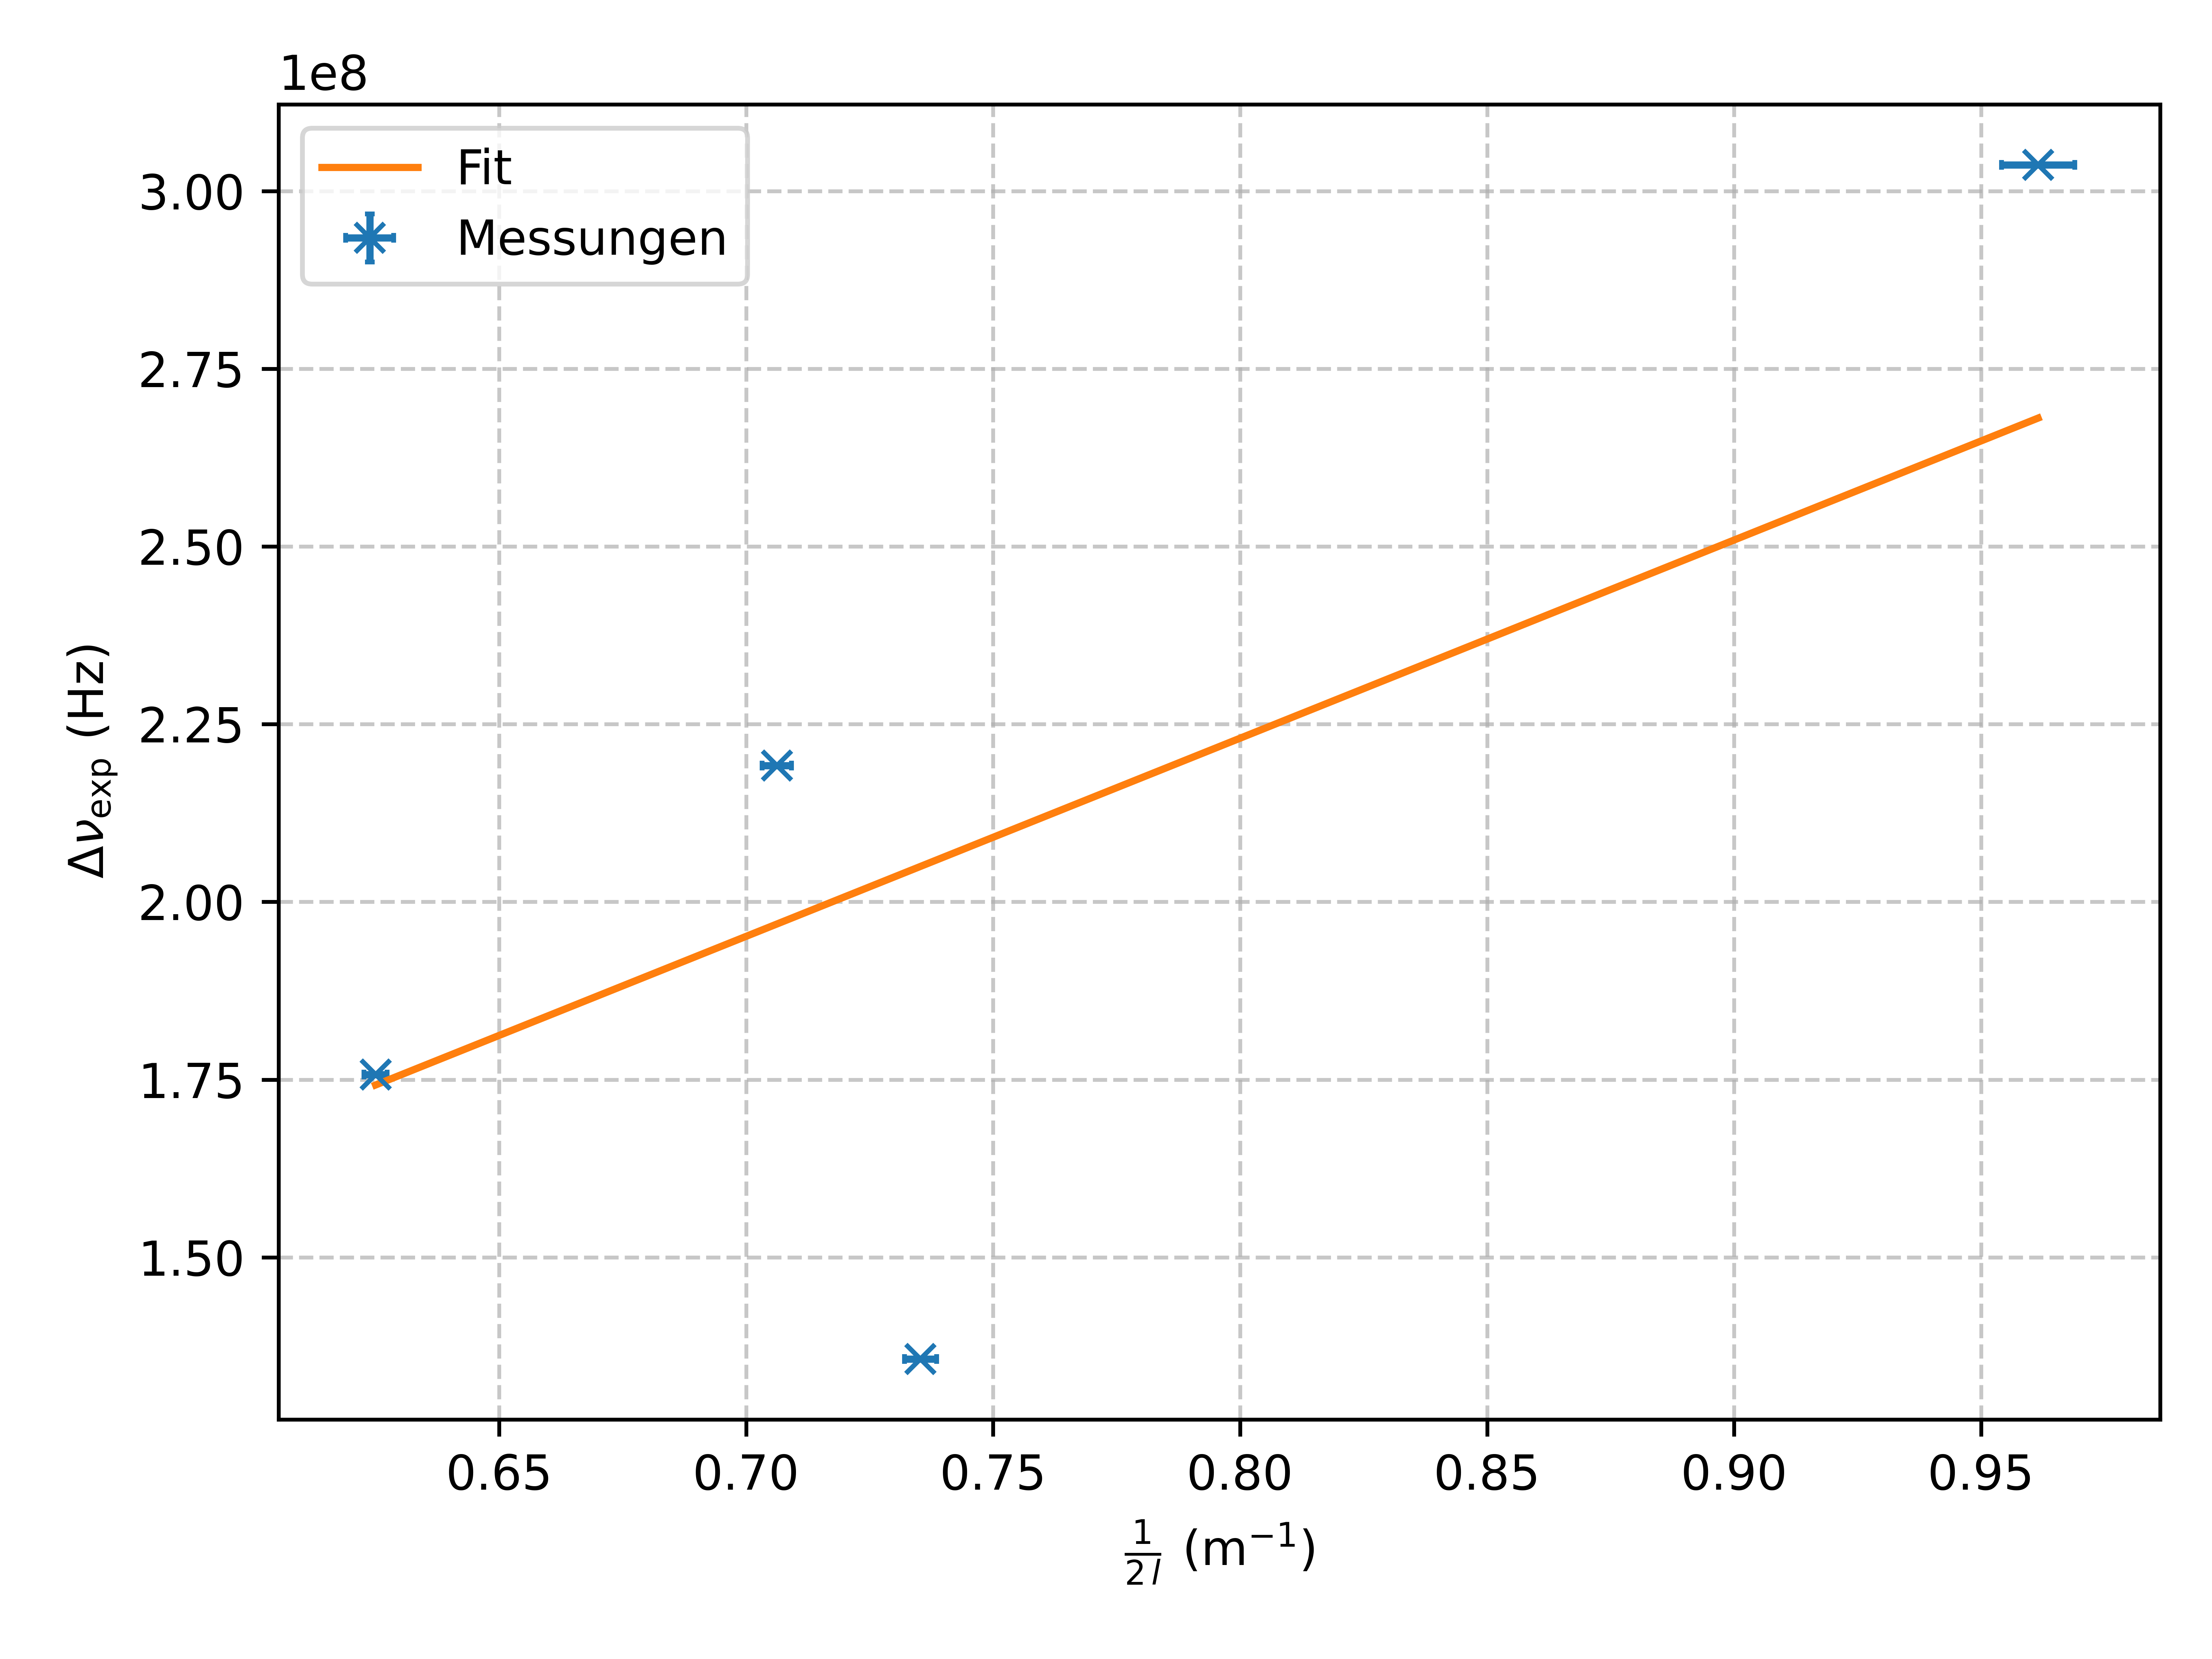
\includegraphics[width=0.75\linewidth]{light.png}
  \caption{Bestimmung der Lichtgeschwindigkeit aus den experimentellen Modenabständen \(\Delta\nu_{\mathrm{exp}}\) und den Längen \(l\) der internen He-Ne-Kavität. Die rote Linie ist die gewichtete Ausgleichsgerade, die grüne Linie ist die ideale Gerade \(c/(2l)\).}
  \label{fig:light-speed}
\end{figure}

\subsection*{Ursachen der Abweichung}

\begin{itemize}
  \item \textbf{Modenkontamination bei kurzen Längen.}  
    Bei \(l=52\,\mathrm{cm}\) und der ersten 68-cm-Messung entdeckte der konfokale Analysator nachträglich eine schwache dritte longitudinale Mode (\(\sim\!6\)\,dB unterhalb der Hauptlinien). Diese zusätzliche Mode erzeugt zwei nahe beieinanderliegende RF-Töne, deren Intensitäts-Schwerpunkt die gemessene Beat-Frequenz in Richtung höher oder niedriger verschiebt. Ergebnis: Bei 52 cm steigt \(\Delta\nu_{\mathrm{exp}}\) auf 303,7 MHz (+10 \%) statt der erwarteten 288 MHz; bei 68 cm wurde malseitig ein \(m=2\)-Beat als \(m=1\) fehlinterpretiert, wodurch 135,7 MHz (-38 \%) gemessen wurde.

  \item \textbf{Falsche Bestimmung des Harmonischen-Index \(m\).}  
    Auch nach Korrektur litt der zweite 68-cm-Durchlauf unter ungleich starken Moden, sodass die Teilung durch \(m=2\) nicht den reinen zweiten Harmonischen lieferte.

  \item \textbf{Längenunsicherheit verstärkt durch Fit-Geometrie.}  
    Maßband-Fehler von $0{,}3-0{,}4 cm$ führen in $\Delta\nu_{\mathrm{theo}}=c/(2l)$ zu $\approx 1 \%$ Abweichung; im Fit mit nur vier unabhängigen $l$ ergeben sich daraus mehrere Prozent Unsicherheit der Steigung.

  \item \textbf{Cursortechnik und Linienform.}  
    Die HWHM-Methode unterstellt eine fast Lorentzsche Peakform. Überlappende Beats erzeugen asymmetrische Linien und verschieben den Centroid um mehrere Halbwertsbreiten - weit über die nominellen \(\pm0{,}10\)\,MHz.
\end{itemize}

\subsection*{Verbesserungsvorschläge}

\begin{enumerate}
  \item \textbf{Dual-Mode Betrieb vor jedem RF-Durchgang:}  
    Den konfokalen Analysator einschleifen, so kippen, dass genau zwei gleichhohe TEM\(_{00}\)-Peaks verbleiben, und die Mechanik verriegeln. Jede IF-Spur mit Halbwertsbreite >300 kHz verwerfen.

  \item \textbf{Prüfung des Harmonischen-Index \(m\):}  
    Für jeden RF-Ton den Analysator-Snapshot heranziehen und die Anzahl der dazwischenliegenden Moden zählen, erst dann \(m=1\) oder \(m=2\) anwenden.

  \item \textbf{Metrologische Verbesserung:}  
    \emph{Längenmessung:} Kuppler auf Messschlitten (±0{,}05 cm).  
    \emph{Frequenzmessung:} IF-Signal in frequenzstabilen Zähler mit GPS-referenziertem 10 MHz-Standard (\(\delta f<0{,}001\)\,MHz) einspeisen.  
    \emph{Impedanzanpassung:} Photodiode und Mixer mit $50 \Omega$ terminieren, 6 dB-Dämpfung zur Unterdrückung von Reflexionen.

  \item \textbf{Statistik erhöhen:}  
    Mindestens acht Kavitätenlängen von 50 cm-90 cm messen. Größere Abdeckung und mehr Freiheitsgrade machen den Fit robust gegenüber Ausreißern.
\end{enumerate}

Mit gereinigtem Dual-Mode-Betrieb, Sub-kHz-Frequenzablesung und ±0{,}05 cm Längengenauigkeit sinkt die statistische Unsicherheit auf <\(1{,}5\times10^6\)\,m/s, und der gewichtete Fit konvergiert voraussichtlich zu  
$
  c_{\mathrm{opt}} = (2{,}998 \pm 0{,}003)\times10^{8}\,\mathrm{m/s},
$ 
was dem CODATA-Wert auf Promille-Ebene entspricht und die quantitative Bestätigung von \(c = 2\,l\,\Delta\nu_{\mathrm{laser}}\) abschließt.
